\documentclass[English]{style/ic-tese-v3}

\usepackage[latin1,utf8]{inputenc}

\usepackage
%  [pdfauthor={nome do autor},
%   pdftitle={titulo},
%   pdfkeywords={palavra-chave, palavra-chave},
%   pdfproducer={Latex with hyperref},
%   pdfcreator={pdflatex}]
{hyperref}
\usepackage{indentfirst}
\usepackage[T1]{fontenc}
\usepackage{titlesec}
\usepackage{subfig}
\titlespacing{\chapter}{0pt}{0pt}{0pt}

\titleformat{\chapter}%
  {\normalfont\bfseries\Huge}{\thechapter.}{10pt}{}

\titleformat{\chapter}{\normalfont\bfseries\huge}{\thechapter}{10pt}{\huge\bf\vspace{5mm}}
\usepackage{adjustbox}
\usepackage{amsmath}
\usepackage{multirow}
\usepackage{float}
\usepackage{pgfplotstable}
\usepackage{pgfplots}
\pgfplotsset{compat=1.13}
\usepackage{caption}
\captionsetup[table]{skip=5pt}

\begin{document}

% Escolha entre autor ou autora:
\documento{Research Project}

\autor{Erik de Godoy Perillo}
\titulo{Attention as a leverage for Deep Learning}
\orientadora{Prof.a. Dr.a. Esther Luna Colombini}

%\paginasiniciais
\section*{Abstract}
Attention is fundamental for intelligent beings.
It is necessary for filtering the significant volumes of stimuli we constantly receive
and for applying the adequate mental resources to perform tasks.
Deep Learning is currently broadly applied to Artificial Intelligence.
The use of Attention in Deep Learning has been increasingly frequent,
resulting many times in better results.
In this context, this work proposes the study and elaboration of approaches to use Attention in Deep Learning
for more power and efficiency to solve problems in Artificial Intelligence.
We aim at obtaining a framework generically applicable in broad problem classes
such as Computer Vision, Natural Language Processing, Program Composition and others.
%\fimdaspaginasiniciais


\chapter{Introduction}
We continually receive high volumes of multimodal stimuli from both external sources
-- such as visual, auditive signals -- and internal sources -- proprioception, memories et cetera.
It would be very inefficient or even impossible to process all the information with
the same intensity once a significant portion of it is irrelevant for
the task executed at the moment and considering that we have limited cognitive capacity.
When we read, our vision does not focus on all
words equally, but instead on a small subset of the text at a time.
When we are addressing a given subject (in a `'train of thought''), it tends to mediate the focus
in the memory search process, essentially retrieving memories that
are useful whereas many other irrelevant memories are not used.
It often happens that something conspicuous
-- such as a bird abruptly appearing in front of us or a sudden sound --
quickly draws our focus, `'stealing'' it from what was previously being focused.
The abilities to filter and select stimuli that are relevant for a task, to keep the focus for an
extended period and to adequately direct mental processes is fundamental to
human beings and other sophisticated forms of life.
We name this set of abilities `'Attention''~\cite{ref:esther-thesis}.

Attention can potentially play an essential role in Artificial Intelligence (AI).
The pursue of intelligent machines is an old effort in Computer Science~\cite{ref:turing} and is still very
relevant today due to the potential to radically benefit society.
Although there have been significant advancements in the field of AI, it is broadly accepted that
machines still cannot perform certain complex tasks nearly as efficiently as humans or some animals and
the path to achieving more intelligence is still unclear, with many different proposals~\cite{ref:mikolov}.
Part of the problem comes from the difficulty to properly define `'intelligence'' itself, but
surveys of the works on the subject~\cite{ref:aidef} suggest that a reasonably accepted
concept is the ability to perform elaborate tasks in complex and dynamic environments
in order to achieve a wide variety of goals.
From the narrow to the broader aspects of intelligence, the functionalities of Attention
are of great importance -- and it increases
as the level of intelligence considered increases~\cite{ref:helgason}.

A considerable amount of advancements in AI in recent years comes from
the popularization of Deep Learning (DL)~\cite{ref:dl}.
As we will discuss in the following sections, the technique mostly consists of
artificial neural networks architectured in a hierarchical manner.
DL showed to be effective in a variety of tasks in Computer Vision~\cite{ref:imagenet}\cite{ref:segmentation},
audio processing~\cite{ref:wavenet} and Natural Language
Processing (NLP)~\cite{ref:att-all-you-need}, mainly due to its ability
to learn what features should be extracted (rather than relying on hand-crafted features).
Along with the transposition from classic models to DL
approaches, an increasingly high number of works on the field
have been using concepts related to Attention in combination with DL to achieve better results.
One example is image captioning (figure \ref{fig:description}) where the task
consists of giving a natural language description of a given image.
The work presented in ~\cite{ref:img-captioning} shows that the task benefits from
sequentially focusing on different parts of the image in a sequence,
through the use of an attentional component in the model.
Other examples -- which will be discussed in-depth in following sections -- include linguistic
translation~\cite{ref:translation}, audio recognition~\cite{ref:audio} and neural computation~\cite{ref:ntm}.
These are evidence that concepts of Attention have indeed been useful for the field.

\begin{figure}
\begin{center}
	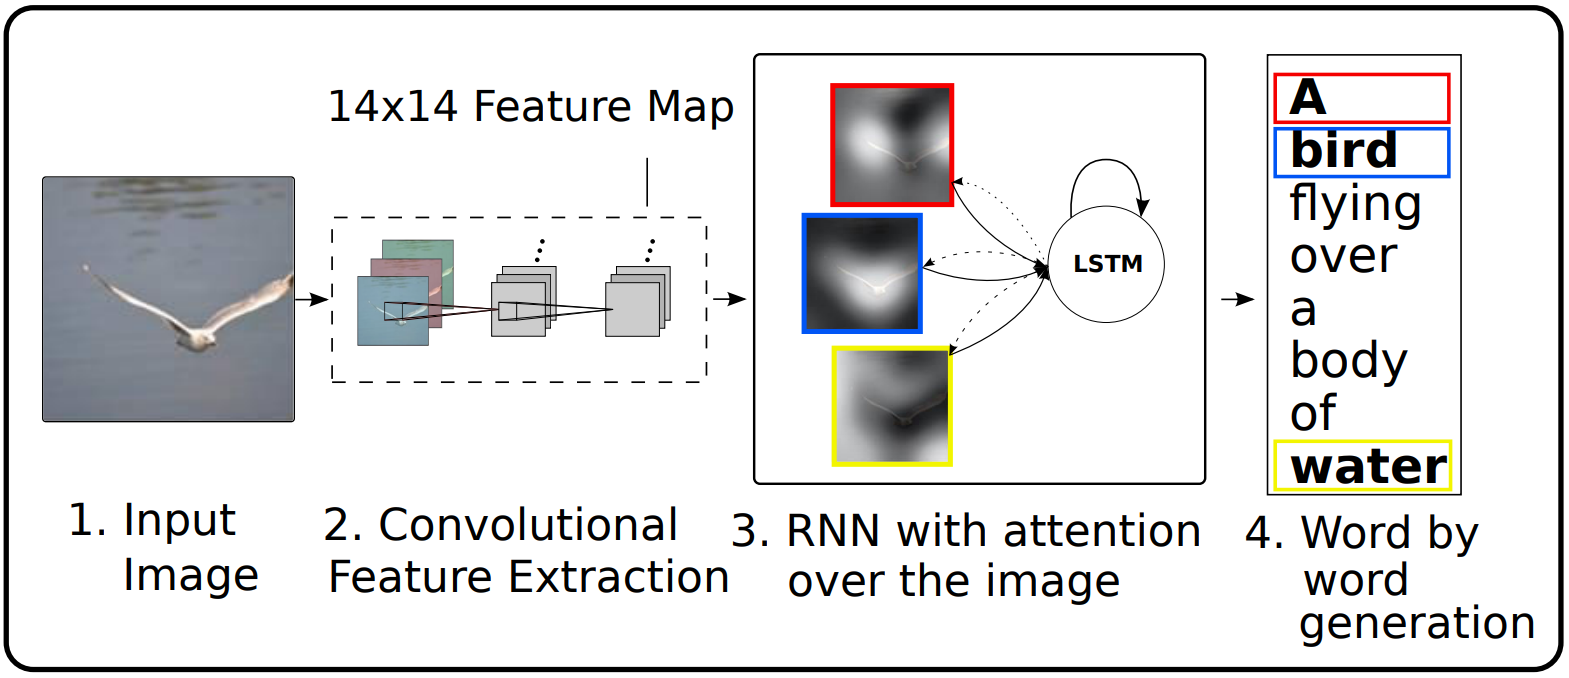
\includegraphics[width=0.9\linewidth]{./img/img_captioning.png}
\caption{
    Diagram of natural language image description using Attention
    (from \cite{ref:img-captioning}).
}
\label{fig:description}
\end{center}
\end{figure}

\section{Motivation and Objectives}
In spite of the recent adoption of Attention by a variety of Deep Learning models
and the significant improvements it has shown, it is conjectured that there are still many other tasks
that are still not very well explored.
Current works also tend to focus more on the filtering functionality of Attention,
but there are other aspects
-- such as the allocation of mental resources in the course of time -- that can be of potential benefit
(we further discuss the taxonomy of Attention in following sections).
Furthermore, we note that Attention models currently being used
are very specific to each problem in question.
Some works propose a higher level of generalization~\cite{ref:recurr-models},
but we believe it is possible to go further.
Therefore, the specific objectives of this work are:
\begin{itemize}
    \item To perform an extensive literature review on the use of Attention
        in modern Deep Learning;
    \item To identify theoretical aspects of Attention itself from areas such as psychology and neuroscience;
    \item To establish general aspects of Attention to be applied to Deep Learning;
    \item To identify specific problems in different classes
        (robotics, vision, natural language, program composition) with
        improvement potential by the use of Attention;
    \item To propose and implement one or more solutions based on the findings of the work in order to
        validate the ideas and evaluate them in an application.
    %\item To study the viability of generalization of Attention
    %    to broader areas in AI other than Deep Learning.
\end{itemize}

The main contribution of the work proposed is related to the first four items:
we wish to
\emph{establish a theoretical framework of Attention as a series of components
    and its applicabilities to Deep Learning.}
Recent works show that the effort on establishing more general concepts and frameworks for
Deep Learning design have been broadly useful.
Examples include the ideas of \emph{Curriculum Learning}~\cite{ref:curriculum}
and \emph{Generative Adversarial Networks}~\cite{ref:gans}.

\chapter{Background}
\section{Attention}
\label{attention}
The interest in the concept of Attention exists since a long time ago.
Throughout the years, Attention has been studied
from various perspectives~\cite{ref:esther-thesis}
such as philosophy, psychology, and neurology.
There are multiple definitions of the concept.
In the next items, we discuss some concrete aspects related to Attention.

\subsection{A definition}
We can define Attention as
\emph{the act of applying mental resources to selected stimuli following an allocation policy specific to
    a particular goal}.
This rather broad definition captures well the main concepts related to Attention:
in a world with virtually infinite
\emph{stimuli} to select from the environment, agents with otherwise \emph{finite processing
resources} (but with a variety of options of \emph{mental processes} to perform) must choose what their
actions will be (and in which stimuli) in a \emph{correct sequential manner} and in \emph{sensible time}.
As mentioned before, other works may define Attention in a different manner
that is perhaps even conflicting with ours but
these are the terms that we choose our work to be based on -- noting that they
reasonably capture common concepts of interest by us and other works.~\cite{ref:helgason}

\subsection{Functionalities of Attention}
Attention can be manifested in different manners depending on the goal.
The most notable functionalities shown in intelligent beings are:
\begin{itemize}
    \item \textbf{To select stimuli} such as looking at only a relevent portion of an image --
        to efficiently use resources on relevant information.
    \item \textbf{To sustain focus} on a specific semantic element for a period of time in order to complete
        a task.
    \item \textbf{To guide processing} in a sequential manner that is relevant for a task.
    \item \textbf{To orient resources} to new important stimuli
        -- such as an abrupt noise comming from somewhere --
        or even in alternating the focus to multiple tasks at the same time.
\end{itemize}

\subsection{Bottom-up and Top-down Attention}
Focus may emerge in two fundamentally different manners~\cite{ref:esther-thesis}~\cite{ref:vocus}.
In bottom-up Attention, the act of focusing is involuntarily
started and guided by (usually) external and conspicuous stimuli,
such as a shattering glass that tends to
make us immediately turn our heads towards where the noise came from.
Another example is visual saliency (figure \ref{fig:saliency}):
a glowing red ball suddenly appearing in
your field of vision will probably grab your focus.
In top-down Attention, focus is voluntarily guided by cognition and goals.
If we are talking to someone in a crowded party, for example,
we focus on what the specific person is saying
-- ignoring other people's words -- in order to maintain the conversation.

\begin{figure}
\begin{center}
		\begin{tabular} {cc}
		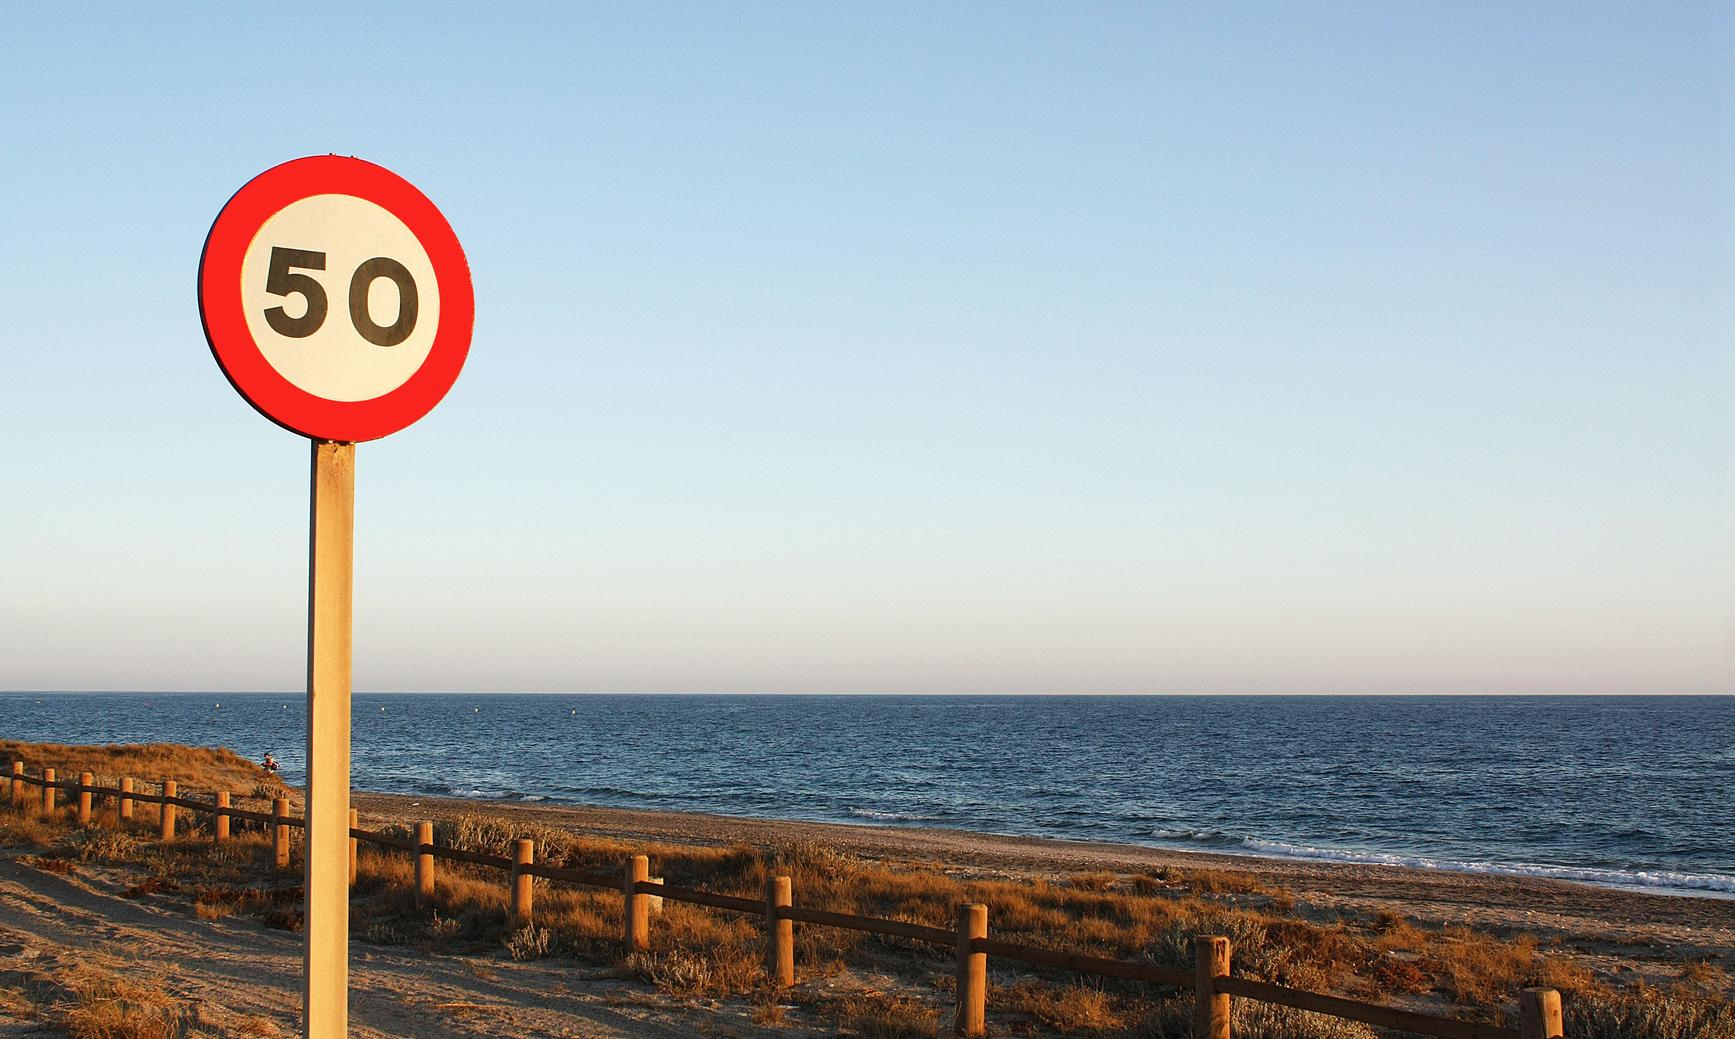
\includegraphics[width=0.40\linewidth]{./img/traffic_sign_s.jpg} &
		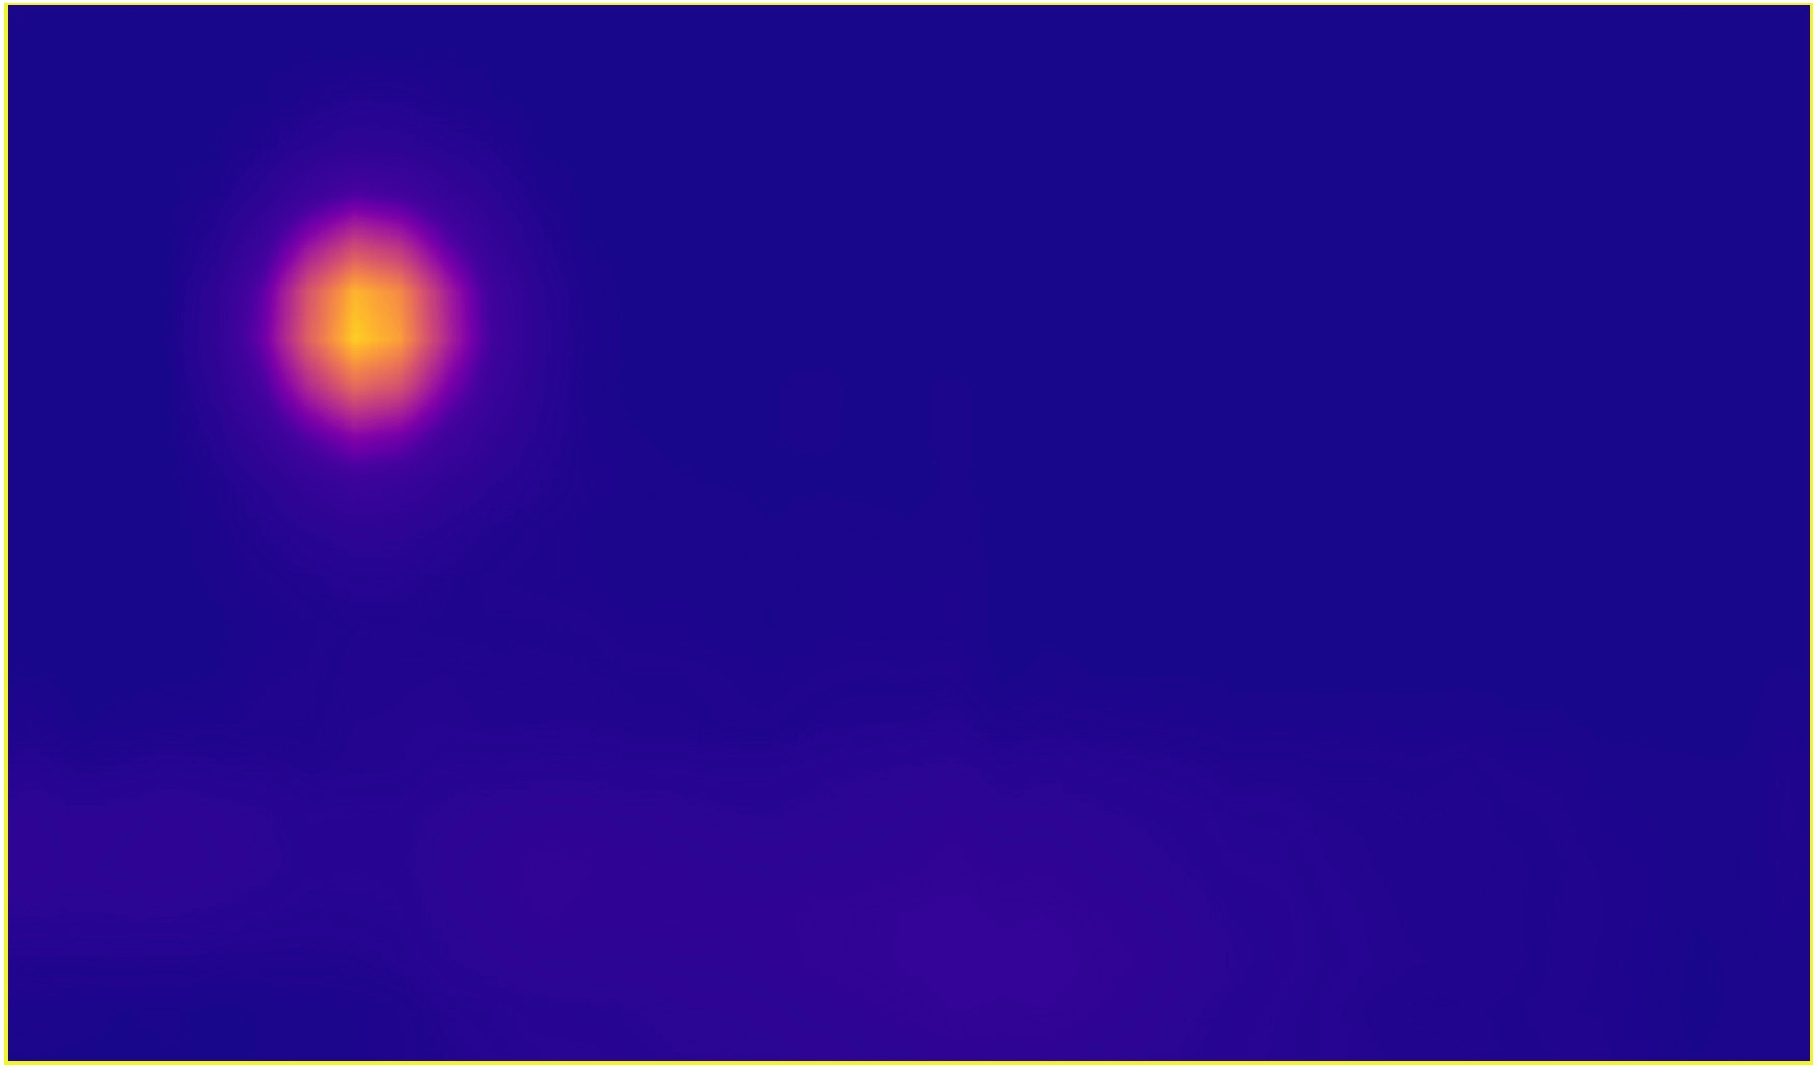
\includegraphics[width=0.40\linewidth]{./img/traffic_sign_m.jpg}\\
        (a) & (b)
		\end{tabular}
\caption{Example of visual saliency.
    b) is the saliency map where higher intensity pixels represent
    regions that are more salient to humans than original image a).}
\label{fig:saliency}
\end{center}
\end{figure}

\subsection{Soft and Hard Attention}
In recent years, there has been an useful distinction between
soft and hard Attention~\cite{ref:att-survey}.
Soft Attention regards defining a continuous distribution of importance
across all elements of information for some task.
In the example of visual saliency, one can determine a saliency map $M$
to a given image $I$ where each pixel will have a value in $[0, 1]$
regarding its saliency.
Hard Attention regards determining a discrete subset of
important information elements.
Using again the problem of visual saliency as an example,
one might want to determine a specific location $(i, j)$ of the image
to be used as center of a small patch of the image that is the most
relevant to be further processed.

\section{Deep Learning}
Deep Learning (DL) is a trend in modern AI~\cite{ref:dl}.
Although DL started being broadly adopted around 12 years ago,
some of its concepts date to much earlier than that~\cite{ref:dl-history}:
foundations of artificial neural networks were already discussed
in the 1950s, backpropagation was introduced in the 1970s
and many other key concepts that are popular mostly in the last decade or less
were introduced more than 30 years ago.
Many fields of AI witnessed a major shift in paradigm
in the last years: models applying DL concepts now achieve state-of-the-art
results in different problems regarding Computer Vision,
audio processing, NLP, neural computation among others~\cite{ref:dl-book}.
DL used used both in supervised and unsupervised learning~\cite{ref:dl}.

One of the key concepts of DL is that of hierarchy of features~\cite{ref:dl}:
A deep sequence of layers apply non-linear transformations to the data
in such a way that many models learn to extract features of hierarchical
levels of abstraction.
For this reason, DL is also regarded as Representation Learning.
This characteristic enables such models to learn latent structure
in intrinsically unstructured data such as images, text and audio signals.
Another advantage is that of transfer learning: models that are
primarily trained for a given task can be used and adapted for another
task while using at least part of the representations learned.
We discuss some concepts related to DL in following items.

\subsection{Artificial Neural Networks}
Artificial Neural Networks (ANNs) are usually adopted to prediction
learning problems by means of learning a non-linear function aproximation.
The ideas used in ANNs date to more than 50 years ago~\cite{ref:perceptron} and many of them
are inspired from observed mechanisms of the human brain.
Most of DL models are a variation of one of the families of ANNs
that will be briefly discussed here.

One of the most basic examples is that of Multi Layer Perceprons (MLPs).
The main caracteristic of this model is the use of hidden layers
and neurons are a linear combination of previous layers followed by
a non-linear activation.
Each layer $l_k$ (with $n$ neurons) is connected to the previous layers
$l_{k-1}$ (with $m$ neurons) and the neuron $l_k^i$, $1 \le i \le n$
is given value:
$$l_k^i = h\left(\sum_{j=1}^{m} l_{k-1}^jw_k^j + b_k^j\right)$$
%Where $h(x): \mathbb{R} \mapsto \mathbb{R}$ is a non-linear activation funcion.
Commonly used activation functions are the sigmoid, hyperbolic tangent
and the Rectified Linear Unit (ReLU):
$$f(x) = \begin{cases}
    0, & x < 0 \\
    x, & x \ge 0 \\
        \end{cases}
$$
ReLU is a currently broadly adopted due to its high efficiency
and training speed~\cite{ref:relu}.

\begin{figure}
\begin{center}
    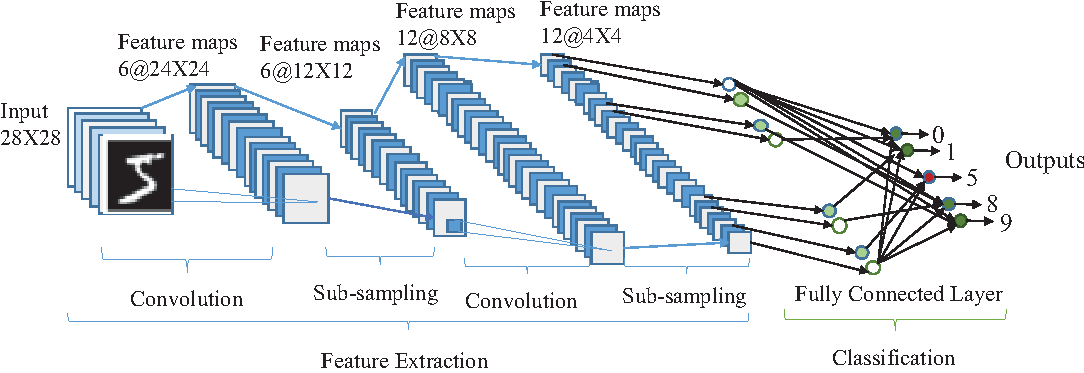
\includegraphics[width=0.9\linewidth]{./img/cnn2.png}
\caption{
    Diagram of a convolutional neural network.
    Learned filters extract features in an increasingly hierarchical manner.
}
\label{fig:cnn}
\end{center}
\end{figure}

\subsubsection{Convolutional Neural Networks}
Convolutional Neural Networks (CNNs) are widely used in Computer Vision
tasks such as image classification, localization and semantic segmentation.
CNNs use the fact that images tend to have correlated pixels and use
convolution filters in an hierarchical manner (figure \ref{fig:cnn})
to learn features in increasing abstraction.
For a certain layer, the $i$-th feature map $m_i$ is,
given filter weights $W_i$, bias $b_i$ and nonlinearity function $h(x)$,
obtained as:
$$m_i = h\left(W_i * x + b_i\right)$$
with $*$ as the convolution operation.

\begin{figure}
\begin{center}
    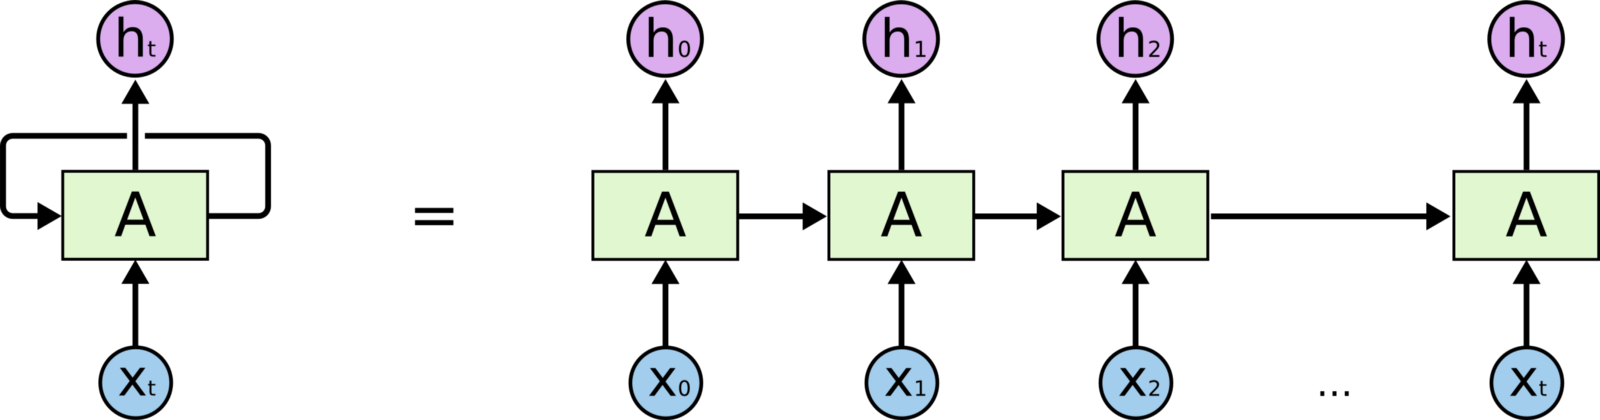
\includegraphics[width=0.9\linewidth]{./img/rnn2.png}
\caption{
    Diagram of a recurrent neural network.
    Time steps map previous outputs and current input to another time step.
}
\label{fig:rnn}
\end{center}
\end{figure}

\subsubsection{Recurrent Neural Networks}
Recurrent Neural Networks (RNNs) are characterized by a recursive architecture
that uses the input of the current step and the output of the previous
step to compute the predictions.
The hidden state $h_t$ at time step $t$, given input $x_t$, weight matrix $W$,
previous state $h_{t-1}$, hidden-state-to-hidden-state matrix $U$ and
non-linearity $f(x)$ is given by:
$$h_t = f\left(Wx_t + Uh_{t-1}\right)$$
These architectures are widely used in NLP tasks such as
machine translation~\cite{ref:rnn-nlp}.
Some variations over the original basic architecture such as
LSTMs are also broadly adopted.

\subsubsection{Modern architectures}
Modern work on Deep Learning propose models of greater complexity than cited above.
Some present completely novice architectures, but most of works tend to be
based on a combination of basic neural networks architectures. The final results, however, may consist
of completely new contributions to new tasks.
Some examples will be discussed in chapter \ref{sess:related-work}.

\subsection{Learning process}
The act of learning the appropriate weights of a given model
is usually obtained by the minimization of a differentiable loss function
that is based on the cost function $L(y, \hat{y})$ that characterizes the error
between the true value $y$ and the predicted value $\hat{y}$.
Backpropagation~\cite{ref:backprop} plays an important role in DL because it's used
to adjust the weights $\theta$ of models that have a
differentiable cost function.
A typical training process is composed of a forward-propagation
step which computes the predictions over a set of input samples
and a backpropagation step which computes the loss function
and adjusts the weights of the model.
In DL, common adjustment methods includes Gradient Descent (GD)~\cite{ref:gd} or variations
which, for a given minibatch, adjusts weights according to:
$$\theta_{i+1} = \theta_i - \alpha\frac{\partial{J}}{\partial{\theta}}$$
where $\alpha$ is the learning rate.

\let\clearpage\relax
\newpage

\chapter{Related Work} \label{sess:related-work}
The topic of integrating Attention concepts into Deep Learning has been increasingly frequent
in the community~\cite{ref:att-survey}.
Augmenting the capabilities of neural network architectures with Attention has shown promising results
in problems from a variety of fields in which Deep Learning is currently being applied to, such as
Computer Vision, Natural Language Processing and differentiable programming in general.
In this section, we address some recent works.
We highlight how Attention was used by the authors and how it affected the performance of the proposed models
on evaluation tasks.

\subsection{Attention-based Encoder-Decoder Networks}
Encoder-decoder networks are a general framework used generally for mapping from input to outputs that both
are of highly-dimensional (often unstructured) data, having being successfully used for tasks such
as machine translation~\cite{ref:enc-dec-rnns}.
One drawback of such architecture is that the encoded feature vector is of fixed size and structure --
regardless of the input -- and not necessarily preserves spatial/temporal structure from the input.
The work in \cite{ref:enc-dec} proposes the usage of an attentional module in between encoder and decoder.
The proposed model's encoder produces feature vectors that have a explicit spatio-temporal structure
(\emph{context set}) of the input and the attentional module uses a relevance evaluation
method to select a subset of the outputs -- either by soft Attention or hard Attention.
This allows the encoder-decoder for more flexibility to select the components of the input that are of
more relevance.
The authors implemented and evaluated the method for several applications:
\begin{itemize}
    \item \emph{Image Caption Generation}: The goal of the task is to provide a natural language description
        of an input image.
        The proposed model uses a CNN as encoder and RNN as decoder -- with the attentional model in between.
        The model was ranked third in \emph{MS COCO Captioning Challenge} and provided highly interpretable
        results regarding the importance of the regions of the image to each component of the sentence
        (see figure \ref{fig:description}).
    \item \emph{Neural Machine Translation}: The authors proposed a RNN architecture
        augmented with the Attention module,
        which provided relative improvement of roughly 60\% when compared to the same model without Attention.
        The model also performs better than state of the art in some languages.
        It was also possible to obtain a weight matrix that maps the importance of input to output words
        since the context set provides structural information of the input (see figure \ref{fig:ntatt}).
    \item \emph{Neural Speech Recognition}: The goal of the task is to translate audio to text sentences by
        using fully neural networks.
        The proposed model uses RNNs between the Attention module and the model achieved state-of-the art
        results in the TIMIT corpus~\cite{ref:timit} and the outputs provide Attention weights from
        the input signal to produced phonemes.
\end{itemize}
Overall, the proposed technique -- besides achieving state of the art results --
produces a semantic mapping from the input space to the output space even when they are of different nature
-- without explicitly being supervised to produce this mapping.

\begin{figure}
\begin{center}
    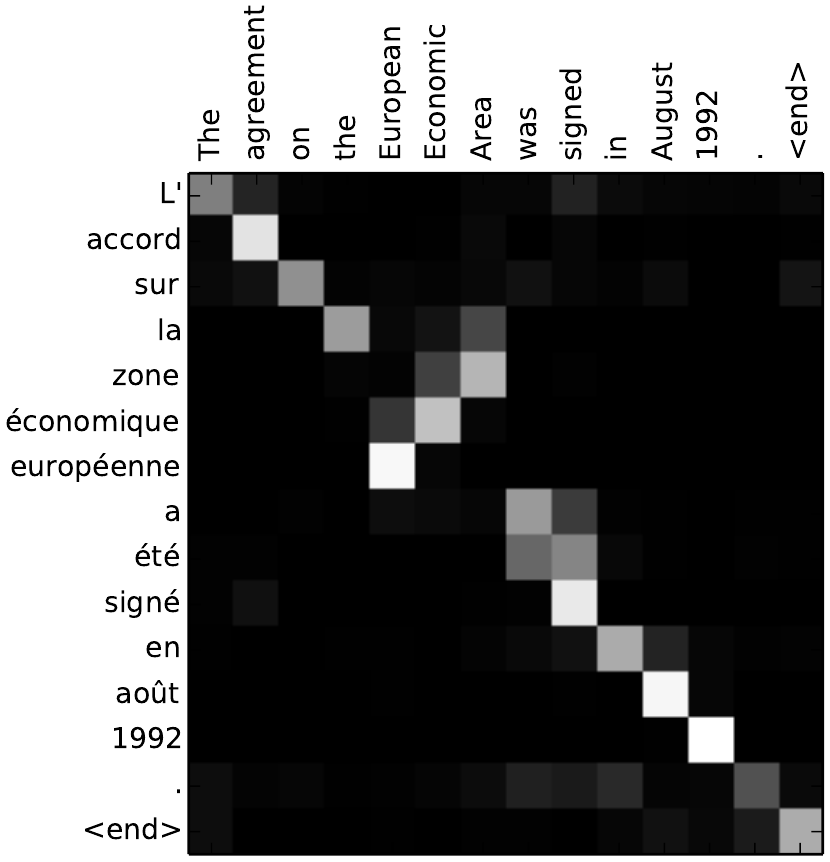
\includegraphics[width=0.5\linewidth]{./img/nt-att.png}
\caption{
    Visualization of Attention weights of the neural machine translation model
    based on Encoder-Decoder networks.
    Figure from \cite{ref:enc-dec}.
}
\label{fig:ntatt}
\end{center}
\end{figure}

\subsection{Adaptive computation time for RNNs}
Most of current works use Attention as a mechanism for filtering.
The authors of the work in \cite{ref:act} propose a RNN augmented with an Attention module that allows for
dynamic inference of number of computation steps for each time step.
It uses soft Attention to determine when to stop (see figure~\ref{fig:adaptive-comp}).
The ability to allocate computational resources is an important functionality of Attention.
The authors show that the mechanism allowed for the model to achieve considerably superior results
in tasks such as adding and sorting (when compared to a model without adaptive computation time)
because the model was enabled to dynamically perform more or less operations depending on the nature
of each step.
The authors also tested the model in the problem of character prediction on the Hutter prize Wikipedia
dataset~\cite{ref:hutter}, in which the model yielded insights into the structure of the input data.

\begin{figure}
\begin{center}
    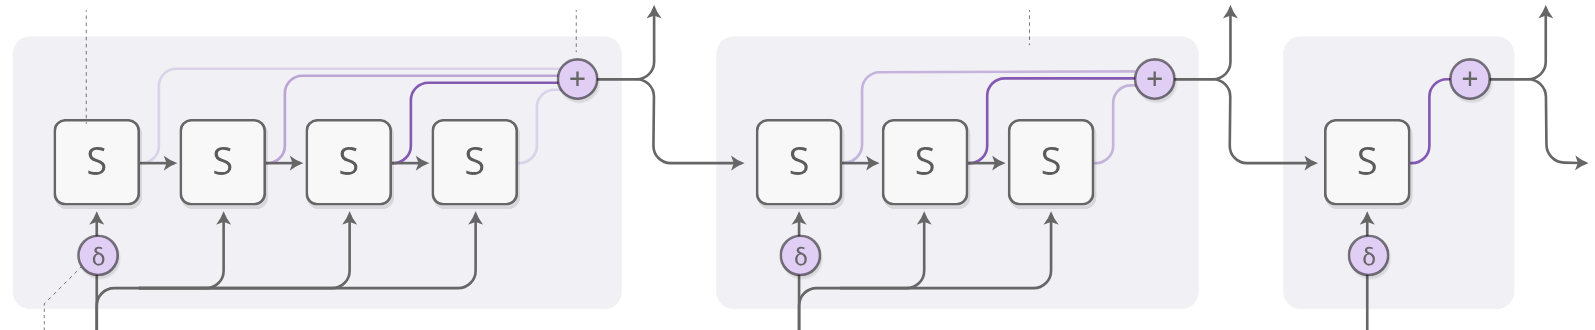
\includegraphics[width=1.0\linewidth]{./img/adaptive_comp.png}
\caption{
    Diagram of the adaptive RNN.
    Each time step can have the amount of computations varied by an Attention distribution.
    Figure from~\cite{ref:distill}.
}
\label{fig:adaptive-comp}
\end{center}
\end{figure}

\subsection{Neural Turing Machines (NTMs)}
Neural Turing Machines~\cite{ref:ntm} are one of the first attempts on building models that can learn to
formulate programs based on DL architectures with continuous cost functions
-- and thus trainable via gradient descent.
The proposed model is composed of a RNN connected to an external memory bank -- which can be read/modified
by the use of read/write heads in the model.
The Attention mechamism is the component that allows for the read and write operations to be differentiable.
On every read/write step, there is an Attention distribution
-- which is updated each step via content-based and location-based methods --
that operates on vectors in the memory locations in a continuous manner.
The authors show that the model is able to learn simple algorithms such as sorting and copying sequences.

\begin{figure}
\begin{center}
    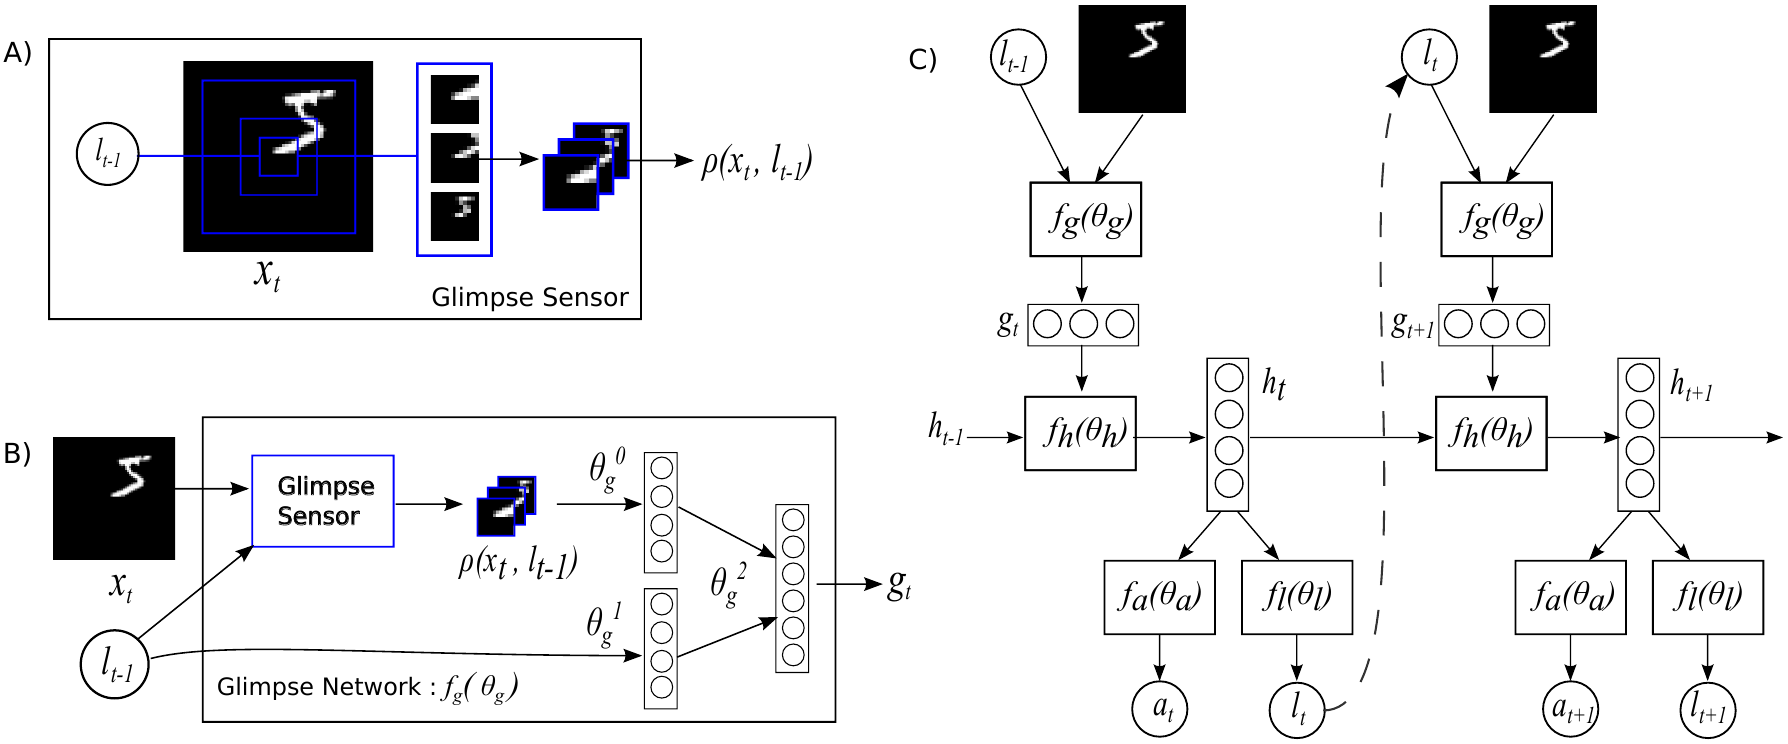
\includegraphics[width=1.0\linewidth]{./img/recurr_model.png}
\caption{
    Overall architecture of the recurrent attentive model.
    \textbf{A)} is the \emph{glimpse sensor} that extracts patches of different resolutions from image
    according to the location being attended.
    \textbf{B)} is the \emph{glimpse module}, which combines information from previous attended locations
    and glimpses to encode a hidden state.
    \textbf{C)} is the RNN architecture augmented with the glimpse module.
    Figure from \cite{ref:rec-models}.
}
\label{fig:recurr-model}
\end{center}
\end{figure}

\subsection{Recurrent Attention Model (RAM)}
The work \cite{ref:rec-models} considers a commonly known problem in Computer Vision: it is usually
expensive to perform processing on images and widely used current models such as
CNNs tend to require computational resources proportional to the number of pixels in the image.
The work proposes a \emph{Recurrent Attention Model (RAM)}, a recurrent neural network augmented by
an attentional component regarded as \emph{Glimpse Module} that is trained via Reinforcement Learning.
The Glimpse Module enables the network to select a point in the image from which it extracts `'glimpses''
-- patches of the image at different resolutions but with the same dimensions.
These glimpes and the selected location are encoded and given as input to produce
the new hidden state of the core RNN architecture (see figure \ref{fig:recurr-model}).
The dimensionality of the glimpes is much smaller than that of the image and furthermore does not depend
on the dimensions of the input image.
The authors evaluate the model for classification tasks in the MNIST~\cite{ref:mnist} dataset and variations
in which the input images are filled more background pixels (resulting in a larger image) and clutter.
The proposed model outperforms a convolutional neural network baseline.
Furthermore, the attentional module in the model enables it to perform the same amount of computation
regardless of the input size of the image and to focus sequentially only at the relevant parts of the image,
which reduces the adversary effect of clutter.

\subsection{Neural Programmer}
Deep Learning techniques have been useful for perception tasks in the last years, but tasks that involve
complex logic and reasoning are still a major challenge.
Authors in \cite{ref:np} propose a model that learns to induce programs by composing basic logic operations
into more complex ones in sequence (figure \ref{fig:np}).
The model is differentiable and thus trainable via gradient descent because the authors use an Attention
distribution at each step to select the operations to be used.
The authors of the work evaluate the model on a synthetic table-comprehension dataset.
The model achieved nearly perfect accuracy and yielded superior performance compared to LSTMs.

\begin{figure}
\begin{center}
    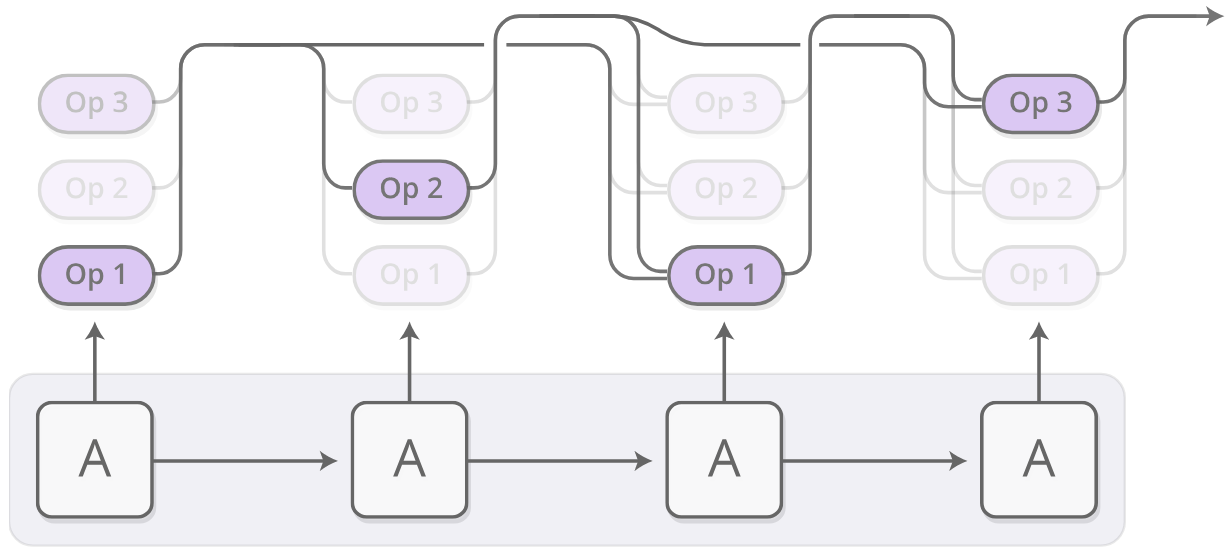
\includegraphics[width=0.7\linewidth]{./img/neural-programmer.png}
\caption{
    Sequence of operations being carried out by the Neural Programmer model.
    Attention distributes the weights to each operation.
    Figure from \cite{ref:distill}.
}
\label{fig:np}
\end{center}
\end{figure}

\subsection{The Transformer architecture}
Sequence models such as RNNs and more specifically LSTMs are broadly used for sequence modeling tasks such
as machine translation.
The work proposed in \cite{ref:transformer} aims at overcoming some challenges inerent to such sequential
models, such as performance and obstacles to apply parallelization to the process.
Complications also arise when the content of the inputs are long (such as long sentences in text) and
recurrent models present difficulties in establishing relationships among words.
The authors present the \emph{Transformer}, an encoder-decoder feed-forward architecture with
Attention as a key element.
The input sentences are embedded and positional encoding is applied.
Then, each layer of the transformer and the decoder employ either \emph{scaled dot-product Attention} or
\emph{multi-head Attention}, which allows for contextual mapping and representation of long-relationships.
The proposed model achieved state of the art results on \emph{WMT 2014 English-to-German} and
\emph{WMT 2014 English-to-French} translation tasks.

\begin{figure}
\begin{center}
    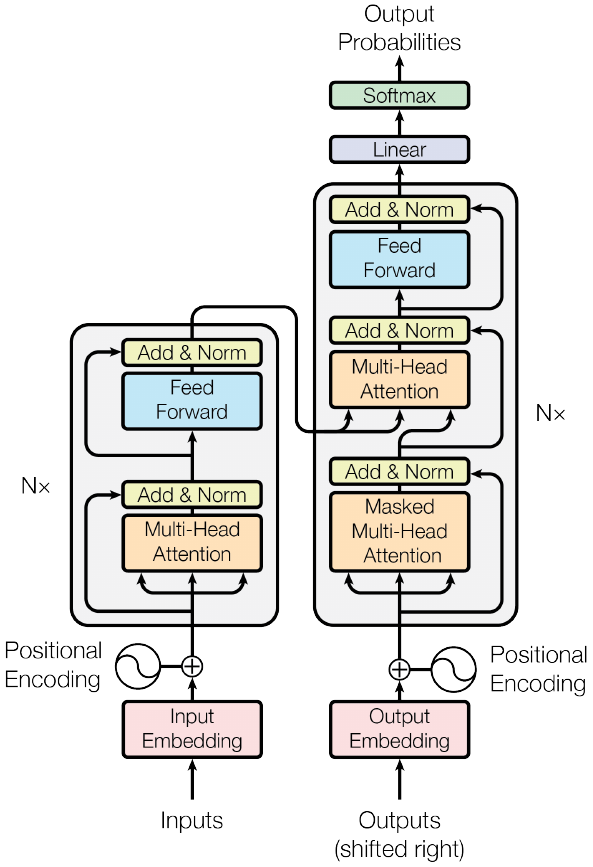
\includegraphics[width=0.4\linewidth]{./img/transformer.png}
\caption{
    The transformer architecture.
    Figure from \cite{ref:transformer}.
}
\label{fig:transformer}
\end{center}
\end{figure}

\let\clearpage\relax
\newpage

\chapter{Methodology}
\section{Activities}
The work can be summarized in three main activities (or \textbf{phases}):
\begin{itemize}
    \item \textbf{1. Literature Review}: an extensive survey on current uses of Attention in modern
        Deep Learning.
    \item \textbf{2. Proposal of an Attention framework for Deep Learning}: \
        from previous activity and further survey,
        devision of a set components of Attention currently used/to be used in Deep Learning design.
    \item \textbf{3. Implementation of Attention in Deep Learning}:
        propose one or more models with components of Attention and carry out evaluations on a set of tasks.
\end{itemize}

The activities to be executed are more specifically described as follows:

\begin{itemize}
    \item \textbf{A1.1 - Theoretical definition of Attention and its components:}
        Using a variety of previous works~\cite{ref:helgason}\cite{ref:esther-thesis},
        we establish a theoretical framework of Attention
        -- extending what was discussed in section \ref{attention} --
        from which we base all future work.
        It is worth noting that this theoretical framework is not necessarily the same as the framework
        we propose to produce specifically for Deep Learning in phase 2.

    \item \textbf{A1.2 - Elaboration of survey:}
        Exploration of selected work under the point of view of the theoretical framework established
        in \textbf{A1.1}.
        For each work, we identify the main components of Attention the authors use, the consequences for the
        performance in the application domain and elaborate a critial evaluation.

    \item \textbf{A1.3 - Survey article writing:}
        Writing of an article with results of phase $2$ to be sent to an appropriate journal.

    \item \textbf{A2.1 - Establishment of Attention components for specific Deep Learning domains:}
        From the theoretical framework obtained in \textbf{A1.1}
        and the exploration of current uses and results in \textbf{A1.2},
        we devise sets of useful components of Attention for specific main problem domains
        in which Deep Learning is broadly used,
        such as image classification, text-to-speech, language translation, image segmentation.

    \item \textbf{A2.2 - Establishment of Attention framework for Deep Learning:}
        From the theoretical framework obtained in \textbf{A1.1},
        exploration of current uses and results in \textbf{A1.2} and
        results from \textbf{A2.1},
        we elaborate a set of components of Attention under a single framework to be applied to more
        general areas of use of Deep Learning,
        such as Computer Vision, Sequence Processing, Program Composition.

    \item \textbf{A3.1 - Arrangement of experiments:}
        From the framework obtained in phase 2, we select a set of problem domains (such as text-to-speech),
        Deep Learning models to use, components of Attention to implement and metrics to evaluate the task.
        The activity aims at selecting all main devised components from phase $2$ in order
        to evaluate the real consequences of their adoption against what was predicted.

    \item \textbf{A3.2 - Execution of experiments:}
        We implement and execute the planned experiments following a pre-defined protocol that
        pays special attention to reproducibility.

    \item \textbf{A3.3 - Evaluation of experimental results:}
        We evaluate the results using established metrics for each experiment,
        elaborating discussions that include interesting aspects of the results in general and
        comparisons between the theoretical predictions and the concrete outcomes.

    \item \textbf{A3.4 - Experiments article writing:}
        Writing of an article with results of phase $3$ to be sent to an appropriate conference.
\end{itemize}

Other activities to be done related to the masters program are:
\begin{itemize}
    \item \textbf{A0.1 - Course's requirement fulfillment.}
    \item \textbf{A0.2 - Qualification Exam.}
    \item \textbf{A0.3 - Masters dissertation.}
    \item \textbf{A0.4 - Defense of masters dissertation.}
\end{itemize}

\subsection{Schedule}

\begin{table}[H]
\centering
\scriptsize
\begin{tabular}{|c|c|c|c|c|c|c|c|c|c|c|c|c|c|c|c|}
	\hline
    \multirow{2}{*}{\textbf{Activity}}
        & \multicolumn{3}{|c|}{\textbf{2018}} & \multicolumn{12}{|c|}{\textbf{2019}}\\
    \cline{2-16}
                  & Oct & Nov & Dec & Jan & Feb & Mar & Apr & May & Jun & Jul & Aug & Sep & Oct & Nov & Dec\\
    \hline
    \textbf{A0.1} & $*$ & $*$ & $*$ &     &     &     &     &     &     &     &     &     &     &     &     \\
    \hline
    \textbf{A1.1} & $*$ &     &     &     &     &     &     &     &     &     &     &     &     &     &     \\
    \hline
    \textbf{A1.2} &     & $*$ & $*$ & $*$ & $*$ &     &     &     &     &     &     &     &     &     &     \\
    \hline
    \textbf{A1.3} &     &     &     &     &     & $*$ &     &     &     &     &     &     &     &     &     \\
    \hline
    \textbf{A0.2} &     &     &     &     &     & $*$ &     &     &     &     &     &     &     &     &     \\
    \hline
    \textbf{A2.1} &     &     &     &     &     &     & $*$ &     &     &     &     &     &     &     &     \\
    \hline
    \textbf{A2.2} &     &     &     &     &     &     & $*$ &     &     &     &     &     &     &     &     \\
    \hline
    \textbf{A3.1} &     &     &     &     &     &     &     & $*$ &     &     &     &     &     &     &     \\
    \hline
    \textbf{A3.2} &     &     &     &     &     &     &     & $*$ & $*$ & $*$ & $*$ &     &     &     &     \\
    \hline
    \textbf{A3.3} &     &     &     &     &     &     &     &     &     &     &     & $*$ &     &     &     \\
    \hline
    \textbf{A3.4} &     &     &     &     &     &     &     &     &     &     &     & $*$ &     &     &     \\
    \hline
    \textbf{A0.3} &     &     &     &     &     &     &     &     &     &     &     & $*$ & $*$ & $*$ & $*$ \\
    \hline
    \textbf{A0.4} &     &     &     &     &     &     &     &     &     &     &     &     &     &     & $*$ \\
    \hline
\end{tabular}
\end{table}

\section{Preliminary Work}
\begin{itemize}
    \item Introduce image classification.
    \item Talk about the problem of getting patches from images.
    \item Introduce visual saliency.
    \item Introduce previous work.
    \item Talk about your experiment.
    \item Talk about results.
\end{itemize}

\renewcommand\bibname{References\vspace*{10mm}}

\begingroup
\let\clearpage\relax
\bibliographystyle{plain}
\bibliography{proposal.bib}
%\printbibliography
\endgroup

\end{document}
